% Wilson's Multi-Asset Research — US Economic Outlook
% Compile with: bash scripts/build_report.sh reports/2026-02-23-us-economic-outlook-economic.tex

\documentclass{wilson-report}

% ── PDF Metadata ──
\hypersetup{
  pdftitle={US Economic Outlook: Late-Cycle Resilience Meets Fiscal Crosscurrents},
  pdfsubject={Macro / Economic Report},
  pdfkeywords={US Economy, GDP, Inflation, Federal Reserve, Fiscal Policy, Strategic}
}

\begin{document}

% ── TITLE PAGE ──
\maketitlepage
  {US Economic Outlook:\\Late-Cycle Resilience\\Meets Fiscal Crosscurrents}
  {Macro / Economic Report}
  {US Economy, Rates, FX, Equities}
  {Strategic (12-Month)}

% ── EXECUTIVE SUMMARY ──
\execsummary{
\begin{itemize}[leftmargin=1.2em, itemsep=4pt]
  \item \textbf{The View:} US economy sustains above-trend growth (\textasciitilde2.0--2.5\% real GDP) through 2026, supported by fiscal stimulus and AI-driven capex, but with rising vulnerability to a late-cycle slowdown by H2 2026. \conviction{M}
  \item \textbf{The Evidence:} ISM Manufacturing surged to 52.6 in January 2026 --- first expansion in 12 months --- while services held at 53.8, signalling broad-based activity. S\&P 500 earnings on track for 13--15\% growth in 2026.
  \item \textbf{The Risk:} Sticky core inflation (\textasciitilde2.5\% CPI, 3.0\% core PCE) constrains Fed easing, while the Supreme Court tariff ruling introduces fiscal revenue uncertainty. A re-acceleration of inflation above 3.5\% would force the Fed to tighten, potentially triggering the recession the soft landing has so far avoided.
  \item \textbf{The Expression:} Favour quality cyclicals and mid-cap industrials over long-duration growth. Prefer short-to-intermediate duration in fixed income. Underweight dollar. Monitor 10Y yield: a break above 4.50\% would signal term premium repricing that challenges equity valuations.
\end{itemize}
}

% ── BODY ──
\section{Macro Context}

The US economy enters 2026 in an unusual position: late-cycle by most traditional metrics, yet with a fresh fiscal impulse that could extend the expansion. The ``One Big Beautiful Bill Act'' (OBBBA), signed July 2025, delivered one of the six largest tax cuts since 1940 (Tax Foundation, Feb 2026). The CBO projects the FY2026 deficit at \$1.85 trillion, or 5.8\% of GDP (CBO, 11 Feb 2026) --- an extraordinary deficit for a non-recessionary economy.

Simultaneously, the Supreme Court struck down President Trump's broad reciprocal tariffs in February 2026, ruling they exceeded emergency-powers authority. This removes a significant inflationary headwind but also eliminates an estimated \$3 trillion in decade-long tariff revenue that was projected to partially offset OBBBA's cost. The net fiscal picture is now more stimulative \textit{and} more uncertain.

\begin{figure}[H]
  \centering
  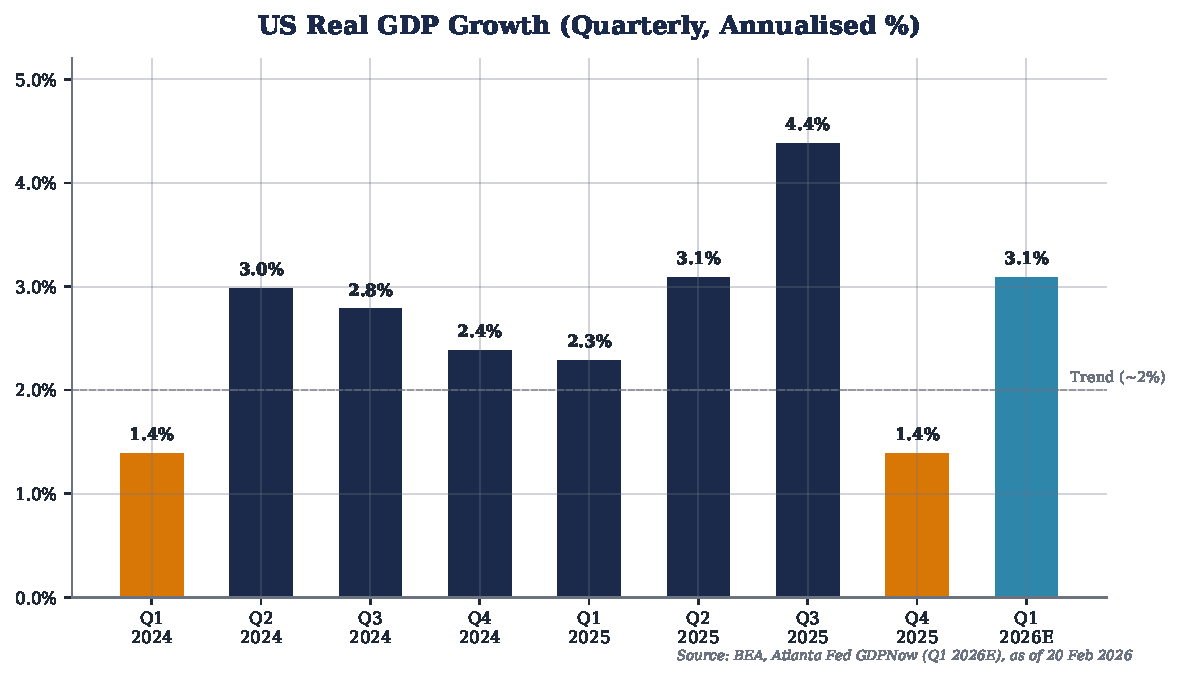
\includegraphics[width=0.95\textwidth]{../figures/us-econ-gdp-growth.pdf}
  \caption{US Real GDP Growth (Quarterly, Annualised). Source: BEA, Atlanta Fed GDPNow, as of 20 Feb 2026.}
\end{figure}

Q4 2025 GDP printed at just 1.4\% annualised --- a notable deceleration from Q3's 4.4\% (BEA, Feb 2026). However, this appears driven by inventory drawdown and the partial government shutdown rather than a fundamental demand collapse. The Atlanta Fed's GDPNow model estimates Q1 2026 at 3.1\%, suggesting a rebound is underway. \textbf{[Measured]}

\textbf{Bridge:} This macro backdrop --- above-trend growth sustained by fiscal stimulus, constrained monetary easing, and a weakening dollar --- creates a specific set of winners and losers across asset classes. The analysis below maps where value, cycle, and sentiment signals converge.

\section{Core Analysis}

\subsection{Growth Assessment: Late-Cycle Extension, Not Early-Cycle Acceleration}

The investment clock places the US in late-cycle territory, but with characteristics that complicate the standard playbook.

\subsubsection{Manufacturing: The January Surprise}

ISM Manufacturing surged to 52.6 in January 2026, the first expansion reading in 12 months after 26 consecutive months of contraction (ISM, 3 Feb 2026). New Orders jumped to 57.1 from 47.4 --- a 9.7-point monthly swing that ranks among the largest on record. \textbf{[Measured]}

\begin{figure}[H]
  \centering
  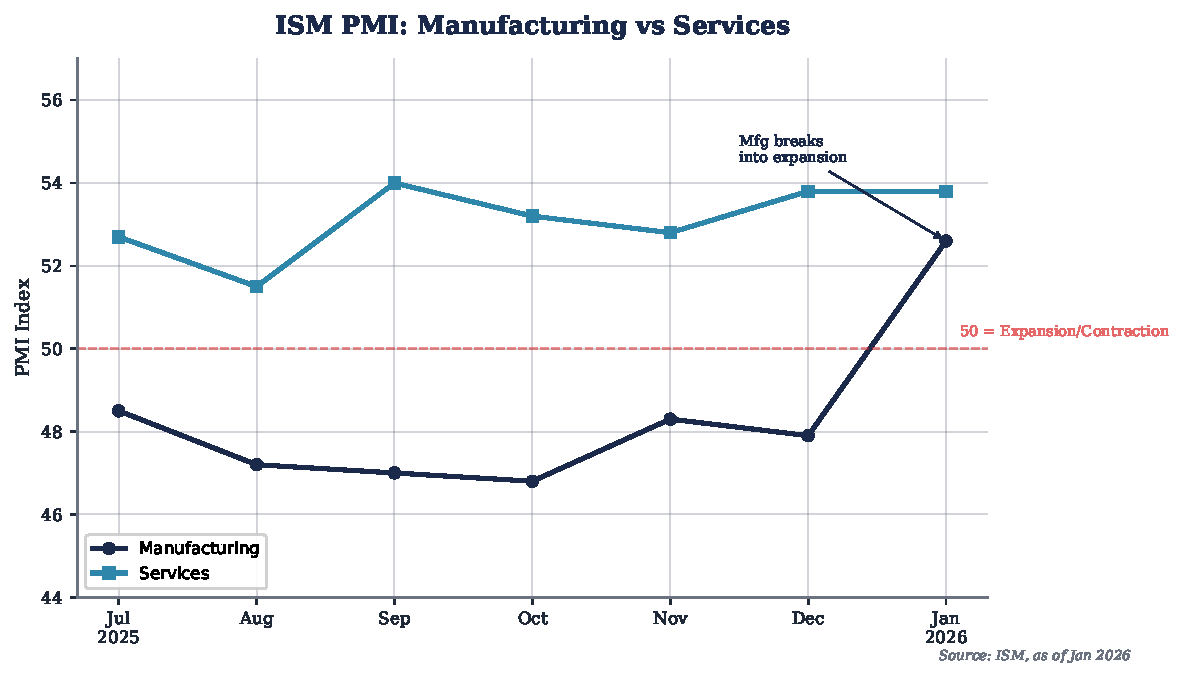
\includegraphics[width=0.95\textwidth]{../figures/us-econ-ism-pmi.pdf}
  \caption{ISM PMI: Manufacturing vs Services. Source: ISM, as of Jan 2026.}
\end{figure}

However, ISM Chair Susan Spence cautioned that January is a seasonal reorder month, and ``some buying appears to be to get ahead of expected price increases due to ongoing tariff issues.'' The S\&P Global flash Manufacturing PMI for February retreated to 51.2 from 52.4, with factory output growth at its lowest since July 2025 and supplier delivery times lengthening to the most since October 2022 (S\&P Global, 21 Feb 2026). \textbf{[Measured]}

\textbf{Our read:} Manufacturing is stabilising, not re-accelerating. The January ISM spike likely overstates underlying momentum due to tariff front-running. But crucially, the sector is no longer contracting --- removing a persistent drag on aggregate growth.

\subsubsection{Services: Steady but Not Accelerating}

ISM Services registered 53.8 in January 2026, matching December and marking the 19th consecutive month in expansion (ISM, 5 Feb 2026). Business Activity rose to 57.4, a healthy reading, but the breadth of expansion has narrowed. \textbf{[Measured]}

\subsubsection{Labor Market: Cooling but Not Cracking}

\begin{figure}[H]
  \centering
  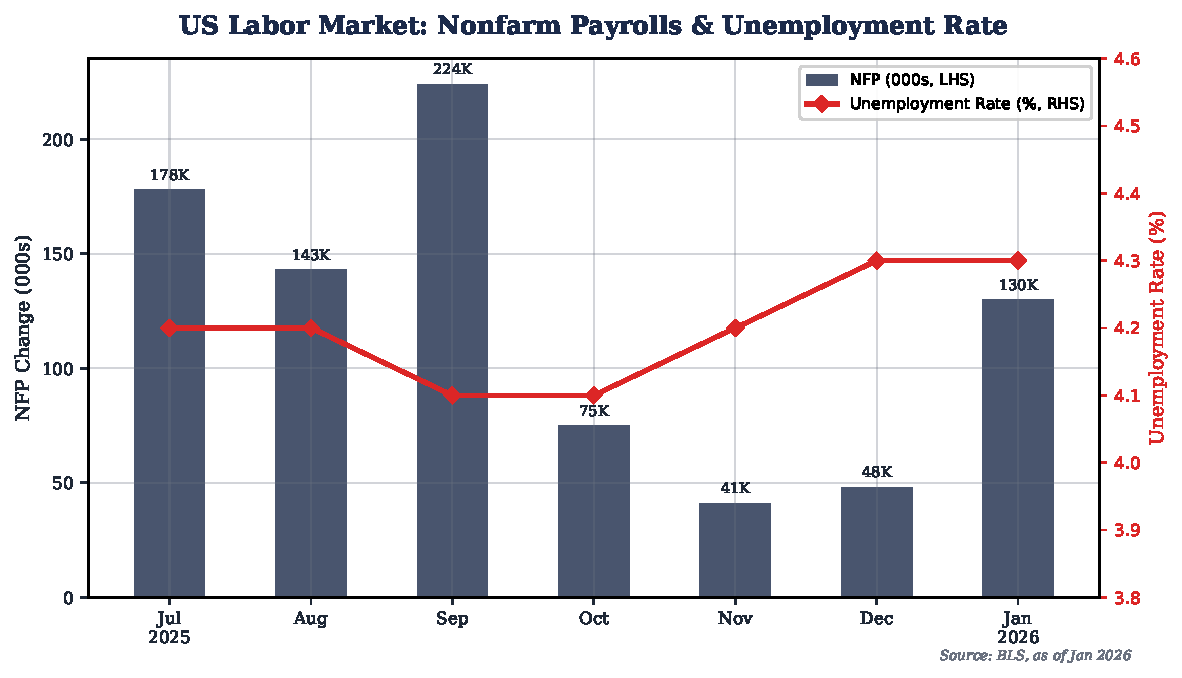
\includegraphics[width=0.95\textwidth]{../figures/us-econ-labor.pdf}
  \caption{US Nonfarm Payrolls and Unemployment Rate. Source: BLS, as of Jan 2026.}
\end{figure}

January nonfarm payrolls rose 130K --- a stabilisation after the volatile Oct--Dec period (75K, 41K, 48K). The unemployment rate held at 4.3\%, up from 3.7\% a year earlier but well below levels that would indicate recession. Hiring is clearly slower, but layoffs remain low. \textbf{[Measured]}

The critical question: is the labour market soft-landing or pre-recessionary? We weight the former. Initial claims remain subdued, the quits rate has stabilised, and the OBBBA's fiscal impulse --- particularly the expanded standard deduction and business tax provisions --- should support consumption and investment through 2026. \textbf{[Inferred]}

\textbf{So what?} The growth picture supports mid-cycle positioning in equities (quality cyclicals, industrials benefiting from capex) rather than late-cycle defensives. The manufacturing turn, if sustained, favours small/mid-caps and value over mega-cap growth.

\subsection{Inflation Regime: Sticky, Not Spiralling}

CPI is running at 2.4\% YoY with core at 2.5\%, while core PCE --- the Fed's preferred measure --- remains sticky at 3.0\% (BLS/BEA, Jan 2026). This creates a tension: headline disinflation is well advanced, but the ``last mile'' to 2\% remains elusive. \textbf{[Measured]}

Key dynamics:
\begin{itemize}[leftmargin=1.2em, itemsep=2pt]
  \item \textbf{Shelter inflation} continues to normalise but slowly. Owners' Equivalent Rent (OER) is still contributing disproportionately to core.
  \item \textbf{Tariff removal (post-SCOTUS ruling)} should relieve goods inflation pressure over 3--6 months. Import prices were a significant contributor to stickiness in H2 2025.
  \item \textbf{Wage growth} has moderated but remains above levels consistent with 2\% inflation, running at approximately 3.5--4.0\% YoY.
  \item \textbf{ISM Prices Paid} in manufacturing ticked to 59.0 in January (from 58.5), suggesting input cost pressures persist even with tariff uncertainty.
\end{itemize}

\textbf{So what?} The inflation picture argues for a Fed that cuts cautiously --- perhaps 50--75bp more over 12 months rather than the 100bp+ that markets were pricing in early 2025. Short-to-intermediate duration preferred in fixed income. Inflation breakevens remain an underowned hedge if the SCOTUS tariff ruling triggers alternative protectionist measures.

\subsection{Federal Reserve: Constrained Easing}

The Fed Funds rate stands at 3.50--3.75\% (upper bound), having cut 175bp from the cycle peak of 5.50\%. With core PCE at 3.0\%, the real policy rate is approximately 0.5--0.75\% --- mildly restrictive but not aggressively so. \textbf{[Measured]}

The SCOTUS tariff ruling complicates the picture in two ways:

\begin{enumerate}[leftmargin=1.2em, itemsep=2pt]
  \item \textbf{Removes inflationary pressure} from tariffs, which supports the case for further easing.
  \item \textbf{Removes fiscal revenue}, widening the deficit and potentially increasing bond supply / term premium --- which argues \textit{against} aggressive easing.
\end{enumerate}

Market pricing implies 1--2 additional 25bp cuts by year-end 2026, consistent with our base case. The key mispricing risk is that the market underestimates the Fed's sensitivity to fiscal dynamics --- a meaningfully wider deficit could push the Fed to hold rates higher for longer to offset bond supply concerns.

\textbf{So what?} The Fed is unlikely to deliver the deep cutting cycle some still expect. Position for a terminal rate of 3.00--3.50\% rather than sub-3\%. This supports financials over rate-sensitive sectors and argues against aggressive duration extension.

\subsection{Fiscal Policy: Stimulus Now, Questions Later}

\begin{figure}[H]
  \centering
  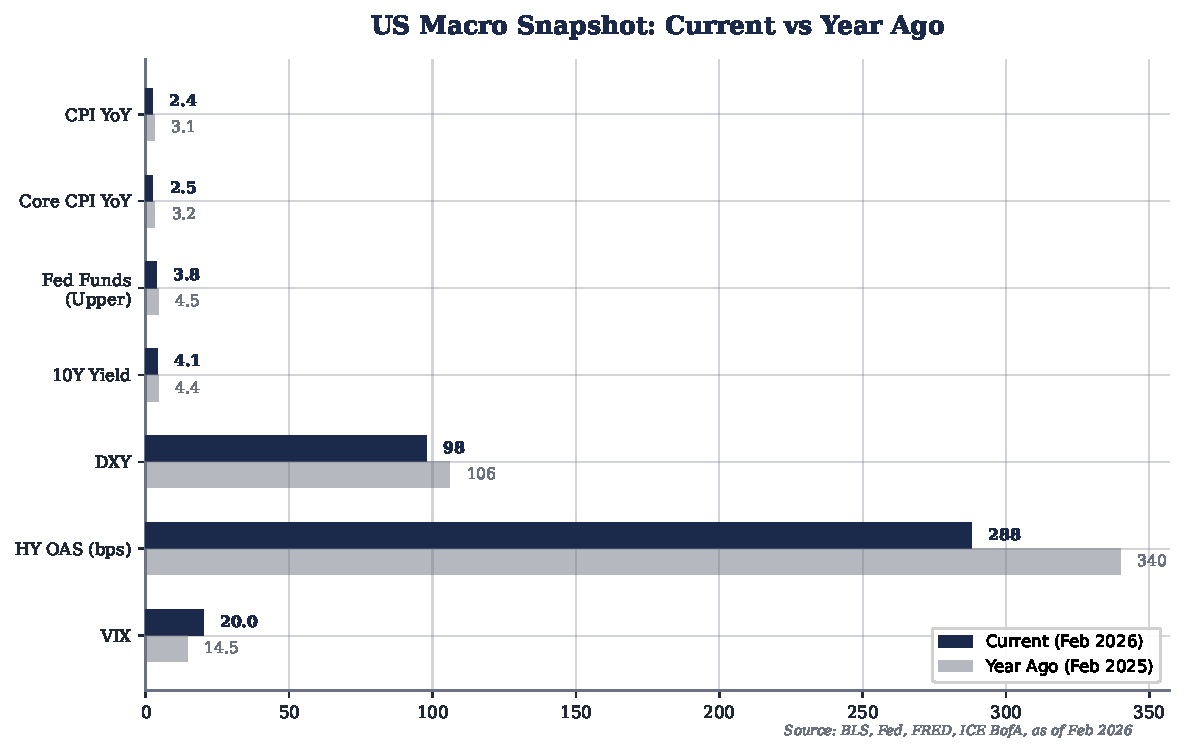
\includegraphics[width=0.95\textwidth]{../figures/us-econ-snapshot.pdf}
  \caption{US Macro Snapshot: Current vs Year Ago. Source: BLS, Fed, FRED, ICE BofA, as of Feb 2026.}
\end{figure}

The OBBBA adds \$4.7 trillion to deficits over the 10-year budget window (CBO, Feb 2026). With the Supreme Court striking down broad tariffs --- which were projected to offset \$3 trillion of that cost --- the net fiscal expansion is now significantly larger. Debt-to-GDP is projected to rise from 101\% to 120\% over the decade, exceeding all historical precedents. \textbf{[Measured]}

Near-term, this is unambiguously stimulative: tax cuts boost after-tax income and business investment. The CBO projects ``real GDP is expected to grow in 2026 as the Republican tax law's provisions begin to outweigh drag from higher tariffs'' (though that projection pre-dates the SCOTUS ruling, which removes both the drag \textit{and} the revenue). \textbf{[Measured]}

The medium-term risk is a bond market repricing of US fiscal sustainability. Net interest costs are projected to more than double to \$2 trillion by FY2035 from \$970 billion in FY2025 (CBO, Feb 2026). Treasury Secretary Bessent's 3\% deficit-to-GDP target now appears unreachable at 6.1\% average over the decade. \textbf{[Measured]}

\textbf{So what?} Fiscal stimulus extends the cycle near-term but builds term premium risk. This is bearish for long-duration Treasuries and structurally supportive of real assets (gold, commodities, TIPS). The DXY at 97.8 --- down 8.3\% YoY --- partly reflects this fiscal deterioration.

\subsection{Sentiment \& Positioning}

Several notable positioning signals:

\begin{itemize}[leftmargin=1.2em, itemsep=2pt]
  \item \textbf{USD bearish positioning} at a 14-year extreme (CFTC, Feb 2026). Despite this, DXY remains range-bound at 96--100. \textbf{[Measured]} Crowded shorts create mean-reversion risk if any data surprises hawkish.
  \item \textbf{S\&P 500 forward P/E} at 21.5x --- above the 5-year average (20.0x) and 10-year average (18.8x), but supported by 13--15\% EPS growth expectations (FactSet, Feb 2026). \textbf{[Measured]}
  \item \textbf{HY spreads} at approximately 288bp --- tight by historical standards, implying minimal recession probability priced into credit markets. \textbf{[Measured]}
  \item \textbf{VIX} at \textasciitilde20 --- elevated from the mid-teens a year ago, reflecting tariff/policy uncertainty. \textbf{[Measured]}
\end{itemize}

\textbf{So what?} Positioning signals caution on the consensus ``soft landing + dollar weakness'' trade. The extreme short in USD is the highest-conviction mean-reversion candidate if data surprises to the upside. Credit markets price almost no recession risk --- if growth disappoints, HY spreads have significant room to widen from current levels.

\section{Scenario Analysis}

\begin{tabularx}{\textwidth}{>{\bfseries\raggedright\arraybackslash}m{1.3cm} >{\centering\arraybackslash}m{1cm} X >{\raggedright\arraybackslash}m{2.4cm} >{\raggedright\arraybackslash}m{3cm}}
\toprule
\rowcolor{BrandNavy} \color{white}\textbf{Scenario} & \color{white}\textbf{Prob.} & \color{white}\textbf{Description} & \color{white}\textbf{GDP / Rates} & \color{white}\textbf{Key Driver} \\
\midrule
\bullrow Bull & 25\% & Fiscal stimulus + AI productivity gains drive 2.5--3.0\% growth. Inflation falls toward 2\%. Fed cuts to 3.0\%. Earnings beat 15\% growth. Dollar stabilises. & GDP 2.5--3.0\%, 10Y 3.75--4.00\%, Fed 3.00\% & OBBBA tax cuts fully flow through; AI capex translates to productivity; tariff removal reduces inflation \\
\baserow Base & 50\% & Above-trend growth of 2.0--2.5\% through H1, slowing in H2. Core inflation sticky at 2.3--2.8\%. Fed cuts 50bp. Deficit concerns simmer. & GDP 2.0--2.5\%, 10Y 4.00--4.25\%, Fed 3.25\% & Fiscal impulse supports growth but fades; labor market cools further; term premium gradually rises \\
\bearrow Bear & 25\% & Fiscal cliff or bond market revolt. 10Y yield spikes above 4.75\% on supply concerns. Financial conditions tighten sharply. Recession by Q4 2026. & GDP 0--1.0\%, 10Y 4.50--5.00\%, Fed holds 3.50\%+ & Bond vigilantes reprice fiscal path; Fed constrained by inflation; consumer weakens as employment deteriorates \\
\bottomrule
\end{tabularx}

\vspace{0.5em}
\textit{Probability-weighted GDP growth: \textasciitilde2.0\%. Subjective estimates informed by data --- not precise forecasts.}

\section{Cross-Asset Implications}

\begin{itemize}[leftmargin=1.2em, itemsep=4pt]
  \item \textbf{Equities:} S\&P 500 earnings growth of 13--15\% provides a buffer against valuation compression. Prefer mid-caps (Russell 2000) over mega-caps on a 12-month horizon --- manufacturing recovery + fiscal stimulus disproportionately benefits domestically-oriented companies. But note: at 21.5x forward P/E, the index needs earnings delivery to justify current levels.
  \item \textbf{Fixed Income:} The 10Y at 4.09\% offers reasonable carry but term premium risk is asymmetric to the upside given fiscal dynamics. Prefer belly of the curve (3--5Y) over long duration. TIPS attractive as inflation hedge given sticky core.
  \item \textbf{FX:} DXY weakness has further to run on fundamentals (twin deficits, rate differentials narrowing) but 14-year extreme short positioning creates tactical squeeze risk. Net: structurally bearish USD, but with hedged exposure.
  \item \textbf{Commodities:} Gold benefits from dollar weakness + fiscal profligacy + central bank demand. Copper supported by AI data centre buildout + manufacturing stabilisation.
  \item \textbf{Credit:} HY at 288bp OAS prices near-perfection. Risk/reward asymmetric to the downside. Prefer IG over HY on a risk-adjusted basis.
\end{itemize}

\section{Risks to the View}

\begin{enumerate}[leftmargin=1.2em, itemsep=4pt]
  \item \textbf{Inflation re-acceleration.} If the SCOTUS tariff ruling triggers alternative protectionist measures (quotas, executive orders) or if wage growth re-accelerates, core PCE could push back above 3.5\%, forcing the Fed to pause or reverse cuts. \textit{Probability: 15\%.}
  \item \textbf{Bond market dislocation.} The \$1.85 trillion deficit without tariff revenue offset could trigger a gilt-crisis-style repricing of US fiscal credibility. 10Y above 5\% would materially tighten financial conditions. \textit{Probability: 10\%.}
  \item \textbf{AI capex disappointment.} Hyperscaler capex is projected at \$539B in 2026 (Goldman Sachs). If AI monetisation disappoints and capex is curtailed, the earnings growth pillar weakens significantly --- Tech accounts for nearly half of projected S\&P 500 EPS growth. \textit{Probability: 15\%.}
  \item \textbf{Geopolitical shock.} Escalation in Taiwan Strait, Middle East, or Russia-Ukraine that disrupts supply chains and triggers risk-off. Exogenous and unquantifiable, but the current VIX at 20 suggests markets are not pricing significant tail risk.
  \item \textbf{Labor market non-linear deterioration.} The Sahm Rule has not triggered, but the unemployment rate has risen 60bp from its cycle trough. A jump above 4.5\% would shift recession probability materially higher.
\end{enumerate}

\section{Key Indicators to Watch}

\begin{tabularx}{\textwidth}{>{\raggedright\arraybackslash}m{2.2cm} >{\raggedright\arraybackslash}m{1.6cm} X X >{\raggedright\arraybackslash}m{2.2cm}}
\toprule
\rowcolor{BrandNavy} \color{white}\textbf{Indicator} & \color{white}\textbf{Current} & \color{white}\textbf{Confirming} & \color{white}\textbf{Disconfirming} & \color{white}\textbf{Next Trigger} \\
\midrule
ISM Mfg PMI & 52.6 & Sustained >51 for 3+ months confirms manufacturing recovery & Drop <48 signals false dawn; January was one-off & 3 Mar 2026 \\
\midrule
Core PCE YoY & 3.0\% & Decline toward 2.5\% validates Fed easing path & Rise above 3.3\% challenges further cuts & 28 Feb 2026 \\
\midrule
NFP Monthly & 130K & Sustained 100--200K range supports soft landing & <50K for 2+ months or unemployment >4.5\% signals recession risk & 7 Mar 2026 \\
\midrule
US 10Y Yield & 4.09\% & Stable 3.75--4.25\% range supports equities & Break above 4.50\% signals term premium repricing & Ongoing \\
\midrule
DXY & 97.8 & Gradual decline toward 94--96 confirms twin deficit thesis & Spike above 102 signals positioning squeeze or hawkish surprise & Ongoing \\
\midrule
HY OAS & 288bp & Stable <300bp confirms benign credit conditions & Widening >400bp signals credit stress & Ongoing \\
\midrule
S\&P 500 Fwd P/E & 21.5x & Earnings growth delivery (>12\%) supports current multiple & Multiple expansion above 23x without earnings support is fragile & Q1 earnings Apr 2026 \\
\midrule
Atlanta Fed GDPNow & 3.1\% (Q1E) & Q1 >2.5\% confirms rebound from Q4 weakness & Q1 <1.5\% suggests deceleration is structural & Weekly updates \\
\bottomrule
\end{tabularx}

\section{Actionable Conclusions}

\conviction{M} \textbf{Above-trend US growth persists through 2026 but decelerating} --- favour quality cyclicals, mid-caps, and short-to-intermediate duration over mega-cap growth and long bonds.

\begin{itemize}[leftmargin=1.2em, itemsep=4pt]
  \item \overweight\ \textbf{US mid-cap industrials / quality cyclicals} (Russell 2000, IWM) --- beneficiaries of manufacturing recovery, fiscal stimulus, and dollar weakness. Monitor ISM Mfg for confirmation.
  \item \underweight\ \textbf{Long-duration Treasuries (TLT)} --- term premium risk from \$1.85T deficit is asymmetric. Prefer belly of the curve (IEF, 3--5Y).
  \item \overweight\ \textbf{Gold / real assets} --- structural dollar weakness, fiscal profligacy, central bank demand. Gold acts as hedge against both inflation re-acceleration and fiscal dislocation scenarios.
  \item \neutralweight\ \textbf{S\&P 500 broad index} --- 21.5x forward P/E requires earnings delivery. Supported in base case, vulnerable in bear case. Selectivity matters more than beta.
  \item \underweight\ \textbf{HY credit} --- 288bp OAS prices near-perfection. Prefer IG for carry with less downside risk.
\end{itemize}

\textbf{Falsification criteria:} This thesis is falsified if (1) ISM Manufacturing falls below 48 for two consecutive months, suggesting the January reading was a false dawn, \textit{or} (2) the unemployment rate exceeds 4.7\% by mid-2026, indicating the soft landing has failed, \textit{or} (3) 10Y yields breach 5.0\% on fiscal concerns, signalling a financial conditions tightening that overwhelms fiscal stimulus.

\section*{Appendix: AI-Generated Hypotheses}

\aihypothesis{
\textbf{Hypothesis: The SCOTUS tariff ruling is net stimulative for the US economy over 12 months.}
\newline\newline
\textbf{Reasoning chain:} The removal of broad tariffs eliminates (a) a 0.3--0.5pp drag on GDP from reduced trade, (b) an estimated 0.5--1.0pp contribution to inflation from tariff pass-through, and (c) significant supply chain disruption evident in the ISM supplier deliveries sub-index. While the ruling also removes \$3T in projected tariff revenue, the stimulative effect of lower prices on consumption and reduced input costs for manufacturers likely exceeds the fiscal revenue loss in the near term. \textbf{[Speculative]}
\newline\newline
\textbf{Validation requirements:} Monitor (1) import price index over next 3 months --- should decelerate; (2) ISM supplier deliveries --- should normalise below 52; (3) consumer confidence --- should improve on lower prices. If all three confirm, thesis strengthens.
\newline\newline
\textbf{Confidence:} Medium. The second-order effects (alternative protectionist measures, fiscal gap) introduce significant uncertainty.
}

\section*{Open Questions}

\small
\begin{itemize}[leftmargin=1.2em, itemsep=4pt]
  \item Will the administration pursue alternative protectionist tools (quotas, executive orders, IEEPA) following the SCOTUS tariff ruling? This would reintroduce both inflationary pressure and fiscal revenue.
  \item Is the AI capex cycle (\$539B projected hyperscaler spend in 2026) generating genuine productivity gains, or is it a capex bubble that will unwind when monetisation disappoints? The answer determines whether 13--15\% S\&P 500 earnings growth is achievable.
  \item At what yield level does the bond market begin to actively discipline US fiscal policy? The gilt crisis threshold for the UK was approximately 100bp above pre-crisis levels. For the US, a 10Y move from 4.10\% to 5.00\%+ would be the analogous signal.
\end{itemize}

\section*{Sources}

\small
\begin{itemize}[leftmargin=1.2em, itemsep=2pt]
  \item \href{https://www.prnewswire.com/news-releases/manufacturing-pmi-at-52-6-january-2026-ism-manufacturing-pmi-report-302675443.html}{ISM Manufacturing PMI, January 2026 (3 Feb 2026)}
  \item \href{https://www.prnewswire.com/news-releases/services-pmi-at-53-8-january-2026-ism-services-pmi-report-302678227.html}{ISM Services PMI, January 2026 (5 Feb 2026)}
  \item \href{https://www.advisorperspectives.com/dshort/updates/2026/02/02/ism-manufacturing-pmi-strongest-expansion-january-2026}{Advisor Perspectives: ISM Manufacturing PMI Analysis (2 Feb 2026)}
  \item \href{https://money.usnews.com/investing/news/articles/2026-02-11/us-budget-deficit-to-grow-to-1-853-trillion-in-fy2026-cbo-says}{CBO Budget Deficit Projections, FY2026 (US News, 11 Feb 2026)}
  \item \href{https://www.crfb.org/blogs/cbo-estimates-3-trillion-debt-house-passed-obbba}{CRFB: CBO Estimates \$3 Trillion of Debt from OBBBA (Feb 2026)}
  \item \href{https://taxfoundation.org/blog/obbba-debt-deficits-tax-revenue/}{Tax Foundation: OBBBA Impact on Revenue, Deficits, and Debt (Feb 2026)}
  \item \href{https://fortune.com/2026/01/26/trump-big-beautiful-bill-national-debt-crisis/}{Fortune: Big Beautiful Bill and National Debt (26 Jan 2026)}
  \item \href{https://www.goldmansachs.com/insights/articles/the-sp-500-expected-to-rally-12-this-year}{Goldman Sachs: S\&P 500 Expected to Rally 12\% (2026)}
  \item \href{https://www.factset.com/earningsinsight}{FactSet Earnings Insight (Feb 2026)}
  \item \href{https://tradingeconomics.com/united-states/currency}{Trading Economics: US Dollar / DXY (Feb 2026)}
  \item \href{https://www.marketpulse.com/markets/us-dollar-pushes-higher-to-start-week/}{MarketPulse: DXY Positioning Analysis (Feb 2026)}
  \item \href{https://www.mcapitalmgt.com/blog/market-insights-what-2026-could-hold-for-the-sp-500/}{M Capital: S\&P 500 Outlook 2026}
  \item \href{https://realinvestmentadvice.com/resources/blog/2026-earnings-outlook-another-year-of-optimism/}{Real Investment Advice: 2026 Earnings Outlook}
\end{itemize}

\signoff

\end{document}
